\documentclass{article}

% if you need to pass options to natbib, use, e.g.:
%     \PassOptionsToPackage{numbers, compress}{natbib}
% before loading neurips_2018

% ready for submission
% \usepackage{neurips_2018}

% to compile a preprint version, e.g., for submission to arXiv, add add the
% [preprint] option:
%     \usepackage[preprint]{neurips_2018}

% to compile a camera-ready version, add the [final] option, e.g.:
     \usepackage[final]{neurips_2018}

% to avoid loading the natbib package, add option nonatbib:
%     \usepackage[nonatbib]{neurips_2018}

\usepackage[utf8]{inputenc} % allow utf-8 input
\usepackage[T1]{fontenc}    % use 8-bit T1 fonts
\usepackage{hyperref}       % hyperlinks
\usepackage{url}            % simple URL typesetting
\usepackage{booktabs}       % professional-quality tables
\usepackage{amsfonts}       % blackboard math symbols
\usepackage{nicefrac}       % compact symbols for 1/2, etc.
\usepackage{microtype}      % microtypography
\usepackage{graphicx}       % to enable graphics on overleaf.com

\title{Improving K-Means Effectiveness and Efficiency with Initialization Estimates of Cluster Centroids}

\author{%
  Robert T.~Boyer, Ph.D.\\
  \texttt{RobertTBoyer@gmail.com} \\
  % examples of more authors
  % \And
  % Coauthor \\
  % Affiliation \\
  % Address \\
  % \texttt{email} \\
  % \AND
  % Coauthor \\
  % Affiliation \\
  % Address \\
  % \texttt{email} \\
  % \And
  % Coauthor \\
  % Affiliation \\
  % Address \\
  % \texttt{email} \\
  % \And
  % Coauthor \\
  % Affiliation \\
  % Address \\
  % \texttt{email} \\
}

\begin{document}
% \nipsfinalcopy is no longer used

\maketitle

\begin{abstract}
  K-Means is known both for its usefulness in finding clusters of related data as well as its fragility with respect to initialization choices.  This paper introduces a $\sim$$95\%$ more effective and $\sim$$50\%$ more efficient initialization methods, that could eliminate the need for multiple executions of K-Means to find high quality clustering.  To initialize the centroids, it selects a multiple, $m$, of $K$ real data points, computes $(mK)^2$ distances and keeps only the K maximum( minimum( distance ) ) points.  A consequence of this technique enables $O( ln K )$ binary search to find the optimal K on 'linearly' separable clusters.  The effectiveness claim applies both to separable and intertwined clusters although the efficiency is lost on intertwined clusters.
\end{abstract}

\section{Background}

K-Means is an unsupervised learning technique for finding clustering (commonality) among data, where the datasets having N data points are partitioned into K clusters. The K-Means grouping algorithm,  initially proposed by MacQueen\cite{macqueen} and based on the work of Forgy,\cite{forgy} performs a greedy search to reduce the within cluster sum of squares error (SSE) cost function.  After initializing cluster centers, it places each data point in the nearest cluster, re-centers all clusters after each full iteration through the data, and repeats until convergence, when all points remain in the same cluster.  The quality, as measured by the SSE, and the performance, as measured by the \# iterations, of the resulting solution is highly dependent on the initial cluster centers.  

The main challenge is effectively and efficiently initialize the starting centroids.  A perfect initialization for K-Means would initialize the centers such that all points are associated to the best centers on the first pass, achieving a global SSE minimum.  Unfortunately, a second pass is still required to confirm no points shifted between clusters after the centroids are re-computed.  Thus, the minimum number of iterations it two.  Further, a perfect initialization would be able to be performed in O( K ).  Multiple initialization models have been put forth, none yet perfect, upon which this model improves.

\subsection{Existing Initialization Models}

Celebi provides a high-level overview of initialization methods including linear, log-linear, and quadratic time complexity mechanisms and reports on the general cost, performance, and failings of these methods.\cite{celebi}  Common methods include randomly generating synthetic starting points,\cite{ng}\cite{yse} randomly assigning points to clusters at startup,\cite{forgy} randomly selecting K real data points,\cite{macqueen} “take a sample; pick a random point, and then k – 1 more points, each as far from the previously selected points as possible,”\cite{leskovec} and randomly selecting a subset, e.g., $\sim$$10\%$, of the full data and running multiple iterations of the algorithm to find good starting points for the full data set.\cite{bradley}

\subsection{Issues}

It is currently understood that K-means should be run multiple times, given the same size K, to improve the overall results due to different result quality based on different initializations.  Why?  The randomness causes substantial variance.  But, why?  Understanding is primarily done in low dimensionality with relatively few data points that make it easy to grok and for which the ability of the algorithm is most always able to find the optimal solution in little time.  However, conceptualizing high dimensionality spaces is difficult, the complications are poorly understood, and the effects on the K-Means algorithm with more dimensions, points, and clusters are not considered.  Further, performance issues are still inadequately addressed.  The quality and performance issues are tightly linked and are both addressed in this paper.

Consider the contrived example in 2D space, figure \ref{fig:contrived}, as a means to express higher dimensionality issues.  Let the larger circles represent the main clusters (with identical numbers of points), the two smaller circles represent outliers to cluster D, and the vertical curve (line) represents a non-linear division for which initial centroid points on the left will attach to clusters on the left and similarly for the right side.  Now, plan to generate initial points for centroids of each of the K clusters.

\begin{figure}
  \centering
  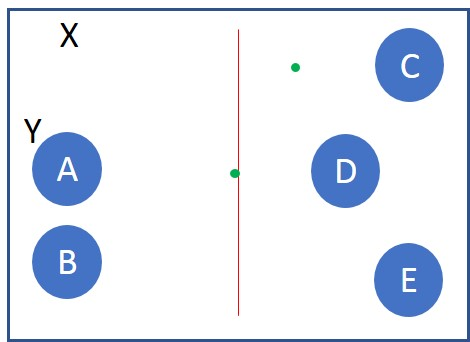
\includegraphics[width=50mm,scale=0.3]{Contrived-3.jpg}
  \caption{Contrived example to discuss initialization method issues in higher dimensions.}
  \label{fig:contrived}
\end{figure}

\subsubsection{Quality Issues}

If randomly generated, synthetic points are used for the centroids, it is easy enough to only have one be generated on the left side (If the curve were exactly in the middle, there would be $5*1/32=5/32$ chance).  With only a single initial point on the left side, the within cluster sum of squares will then be minimized by joining the left two clusters (A + B) and splitting one of the right clusters.  Or, conversely, there is a $50\%$ chance that the left side is given 3 of the starting centroids, also yielding poor results.  Further, consider points X and Y as representing potential centroid initializations, then X is totally occluded by Y.  Empty clusters are the result.

Randomly choosing real points from among the clusters will eliminate empty clusters, but small or single-point clusters could result when nearby points are randomly chosen.  Randomness could easily choose only one point from among the pair of clusters on the left.  With the five clusters, there is only a $4\%$ chance that each cluster is represented.  As the number of clusters increases, the probability of drawing one point from each group further diminishes.

Randomly assigning points to clusters will usually create initial centroids just right of the dividing line.  When applying the K-Means algorithm, most likely only one centroid will be forced to the left with the remainder to the right.  But first, that centroid will attach to C, D, or E and then have to relinquish those points over to other centroids, costing extra iterations

Taking a sample and then selecting $k-1$ additional points as far from the previously selected points as possible is conceptually useful.  However, using the max sum of distances from a potential point to the prior selections will cause the extreme points in the system will be selected, as shown in the large, goldenrod squares in figure \ref{fig:maxiMinMeans}.  The max sum of distances causes internal clusters to be skipped over and allows adjacent points to be selected.  Additionally, it is likely to select outliers in preference to primary points.  In the contrived example, this poses similar risks to the ones described above.
 
\begin{figure}
  \centering
  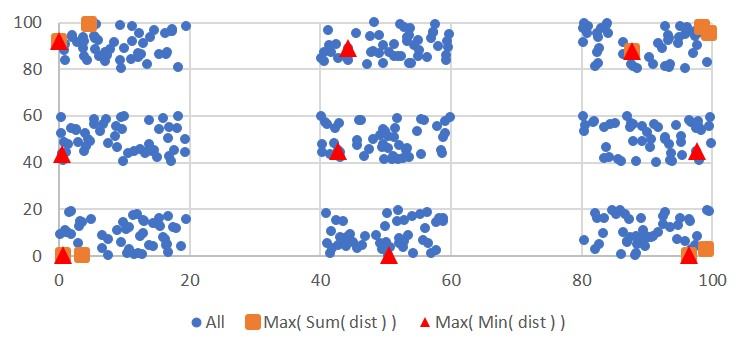
\includegraphics[width=80mm,scale=0.3]{MaxiMinMeans.jpg}
  \caption{Initialization by max( sum( dist ) ) vs max( min( dist ) ) to existing centers.}
  \label{fig:maxiMinMeans}
\end{figure}

\subsubsection{Performance Issues}

In a standard K-Means implementation, each time any centroid is refined, the entire dataset must be re-evaluated.  Thus, as two centroid initializations share points from the same cluster or worse, multiple clusters, then a multi-iteration tug-of-war ensues to find non-overlapping clusters.  As is shown in figure \ref{fig:pointQtyIssue}, the more points per cluster, the slower the movement, the more iterations.  Thus, the "far away" concept is useful as fewer points will be caught by the wrong centroid and will be more easily released.  But, the max sum of distances initialization cost of $NK(K-1)/2$ is effectively $(K-1)/2$ extra iterations of the algorithm.

\begin{figure}
  \centering
  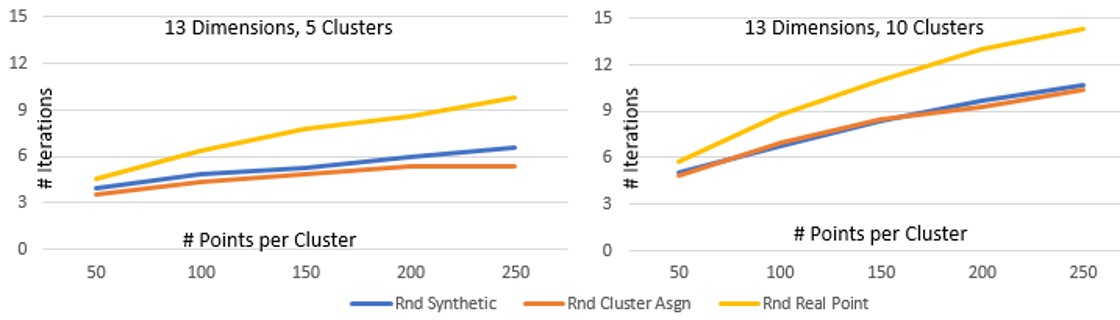
\includegraphics[width=100mm,scale=0.3]{PointQtyIssues.jpg}
  \caption{Increasing points per cluster has a direct effect on the \# iterations.}
  \label{fig:pointQtyIssue}
\end{figure}

\subsubsection{Determining Size of K Issues}

There are many methods to attempt to determine the best number K of clusters.  These include the elbow, silhouette, and gap methods among many others.\cite{UC}  They are predicated on running the algorithm multiple times, $t$, with different values for K (e.g., $k0$ to $kt$) and then analyzing the resultant SSE clustering.  The best K answer is sometimes questionable, especially with the variability of initialization centroids. And, the cost involved is $\sum_{k0}^{kt} Iterations_k * N * k$.  How can the size of K be found efficiently in an unknown space?

The challenges identified in this highly contrived 2-dimension example appear to occur naturally and frequently in higher dimensions, as evidenced by the need to run multiple instances of the algorithm.  Further, the cost to find K may be excessive at scale; more efficient and effective means are required beyond using a subset of the full dataset.

\subsection{New Initialization Methods}

The first approach is a minor adjustment to the "take a sample and then $k-1$ additional points."  Leverage the "far away" concept, but re-define it to be "not near."    Instead of using the maximum of the sum of the distances to previously selected centroids, change the decision criteria to the maximum of the minimum distance between a potential center and the existing centers.  As shown in the red triangles in figure \ref{fig:maxiMinMeans}, this Maxi-Min-Distance (MMD) initialization places points in each cluster, solving the adjacent point problem.  However, the cost factor, effectively $(K-1)/2$ extra iterations, is still an issue as are the risks associated with selecting outliers.

The second approach solves both the initialization cost and placement by providing a more efficient structure to the sampling and the subsequent point selection.   It solves the challenge of selecting points too close to one another.  Also, this approach can be a preliminary action for executing of K-Means on partial data to initialize centroids in preparation for running K-Means against the entire data when working with big data or as a replacement for it.  This new initialization method, “cross-centroid cost maximization,” selects a configurable multiplier $m$ and selects $mK$ random, real data points, independently selected to avoid data ordering issues.  Logically, a two-dimensional, symmetric, square matrix is used to hold the cost relationship between each of the points with a cost O( $(mK)^2$ ).  Then, the maximum( minimum( distance ) ) nodes are kept.  This is implemented as sorting the costs, low to high O( $(mK)^2$ ln( $(mK)^2$ ) ), with the $(m-1)K$ lowest cost, nearest points removed until only the K most costly, furthest points remain for initialization.

The key features are:
\begin{enumerate}
\item Subsampling from the real points has a small probability of choosing an outlier or an empty cluster.
\item Subsampling \textbf{mK} real points increases the probability of choosing at least one point from each of the K clusters, thus accelerating convergence toward intended/actual clusters.
\item Removing the $(m-1)K$ lowest cost points solves the problem of choosing points too close to one another and efficiently solves the “find k-1 distant points.”
\end{enumerate}

When removing one of a pair of nearby nodes (i.e., lowest cost pair), experiments were run with random selection (CCCM-Rnd) and on removal of the minimum cost (CCCM-Min) basis for which of the two nodes to remove.  The results are presented, showing that removing the node with the lowest sum cost, relative to the $mK-1$ other potential nodes, was slightly more effective.

Finally, a third method blends CCCM and MMD.  The $mK$ real points are selected, then MMD is applied to these points, resulting in a cost of O( $mK^2(K-1)/2$ ), which is effectively $mK(K-1)/(2N)$ extra iterations (usually a fraction, e.g., 0.28 extra iterations.  N=50K, m=7, K=5 ==> 28/100).  The current data shows this to be equivalent to the simpler methods.

\subsection{New Method To Determine Size of K}

It is well understood that increasing the size of K reduces the SSE and that increasing K beyond the true number of clusters will have much less improvement.  This is the basis for the elbow method.  But, as observed in the issues section, when multiple centroids 'fight' over the same points, extra iterations are required to resolve the issue.

Analyzing only the number of iterations, looking for a significant uptick in the number of iterations (to a value above 4 for separable clusters), while using CCCM(m=7) provides an reliable estimate of the true K, at least within the synthetic test environment.  Combined with SSE, an O( ln K ) binary search may be formed, thereby reducing the cost to find the best K.

\section{Experiments}
\label{experiments}

Experiments were performed, using both synthetic and real data sets, to analyze three elements: quality, performance, and the ability to determine the best number of clusters K.

\subsection{Initialization Methods}

Each experiment trial used the exact same set of points with different centroid initialization methods.

\begin{itemize}
\item Random \cite{jancey} – randomly generate K synthetic points in the available space.
\item Cluster \cite{forgy} – randomly assign points to a cluster, calculate centroid as starting point.
\item Rnd-Point \cite{macqueen} – randomly select K points from the real data points.  This is equivalent to setting $m=1$ for CCCM below and will be embedded in the result sets below.
\item CCCM-Rnd – randomly select $mK$ points from the real data points, calculate $(mK)^2$ cost values, remove the $(m-1)K$ points having the lowest costs.  As a cost is between a pair of points, randomly select which of the two points to remove.
\item CCCM-Min – same as CCCM-Rnd, but after the minimum-distance pair is selected, remove the point with the minimal overall cost (i.e., sum of cost to all other $mK-1$ points).
\item CCCM-MxMn – similar to other CCCM, but uses MMD to select the points to keep.
\end{itemize}

\subsection{Synthetic and Real Data}

Synthetic data is created in various dimensions, clusters, and point quantities.  Real data from the UCI Machine Learning Repository, the Iris Data Set \cite{UCIIris} with 150 data points with 4 numeric dimensions and 3 clusters and the Mice Protein Expression Data Set \cite{UCIMice} with 1079 data points with 64 numeric dimensions and 8 clusters are used.  Empty data were filled with nearest neighbor values from the same cluster of mice.

\subsection{Smaller K sizes}

\begin{verbatim}
The following was repeated in 3, 5, 7, 9, 11, and 13 dimensions.
  The number of means is set K=2 thru 25, increment by 1
    For each K size, run 25 iterations of creating one cluster per mean 
      Per cluster:
        Randomly create an origin
        Randomly create 50 points
          Distribute values [-10,10] from the origin on each dimension.
      Calculate the intended "best" (optimal) result
      For each of the initialization methods (including m=1 to 7, inc by 1)
        Execute the K-Means algorithm 50 times and average the results.
\end{verbatim}

\subsection{Larger K sizes}

Using only 13-dimensions and K in 50, 100, perform the same test suite as above.

\subsection{Determining K}

\begin{verbatim}
Using 13-dimensions and m=7
  The number of actual clusters is set srcK=2 thru 10, increment by 1
    Per cluster:
      Randomly create an origin
      Randomly create 50 points
        Distribute values [-10,10] from the origin on each dimension.
    Calculate the intended "best" (optimal) result
    For each trial K size, dstK= max(1,srcK-8) thru srcK + 4
      For each of the initialization methods
        Execute the K-Means algorithm
\end{verbatim}

To demonstrate the usefulness of CCCM, 13-dimensions, m=7, and multiple K values are used to provide a graph of the performance of the various initialization methods.  In actual use, one would combine the SSE reduction with the \#Iterations and create a binary search.  The SSE reduces toward optimal K, but then the \#Iterations has a sharp increase after the optimal K.

\section{Results}
\label{results}

For each dimension, the quality and execution performance are tracked.  For synthetic date, the intended best performance of a given set of clusters is calculated as the basis by which to evaluate the various initialization methods.  When clusters overlap (i.e., are not linearly separable), then this "best" value may be larger than the actual value.  Both small and large K size results are shown together.  For presentation purposes, only 13-dimensional data is shown.  For real data, the observed best result (across all initialization models) is used as a reference point for analyzing the quality of results.  As CCCM-Rnd, -Min, and -MxMn are nearly identical, only CCCM-Min is shown.  Also, to reduce clutter, m=2, 4, and 6 have been stripped from the graphs.

\subsection{Quality of Results}

\begin{figure}
  \centering
  \includegraphics[width=\linewidth]{13D-MeanVsOptimal.jpg}
  \caption{Mean as a percentage of the optimal cost.}
  \label{fig:meanVsOptimal13D}
\end{figure}

Figure \ref{fig:meanVsOptimal13D} shows the mean cost compared to the optimal, by initialization method and number of clusters.  At most all K sizes, the mean costs of the existing methods are $200\%+$ over the optimal while CCCM, using $m=7$, is within a few percent over the optimal, yielding an improvement of over $\sim$$95\%$.

\begin{figure}
  \centering
  \includegraphics[width=\linewidth]{13D-StdevAway.jpg}
  \caption{\# stdev the mean is away from the optimal SSE, by initialization method, by K size.}
  \label{fig:stdevAway13D}
\end{figure}

Figure \ref{fig:stdevAway13D} shows how far, in terms of standard deviations, the results of an initialization method are from the optimal clustering.  In part, this shows why multiple executions of K-Means are used to drive down the cost to find the best clustering.  However, it also shows a low probability of finding a good result within just a few repeats of the algorithm.  As K grows, there is a near impossibility of achieving optimal clustering with the older methods, yet CCCM has a much slower growth rate and provides results close to optimal, even with high numbers of clusters.

It also shows the effects of altering the m scalar.  By increasing the multiplier, the probability that all clusters are represented in the original $mK$ selection increases. Then the removal of low-cost pairings helps keep each of the clusters represented.  Incrementing to $m=7$ drives the quality to within a few percent of optimal for both the synthetic data and to within $\sim$$10\%$ for the real data.

\subsection{Execution Performance Results}

\begin{figure}
  \centering
  \includegraphics[width=\linewidth]{13D-AvgNumIters.jpg}
  \caption{Avg \# iterations, Avg \# empty clusters, by initialization method.}
  \label{fig:numIter13D}
\end{figure}

Figure \ref{fig:numIter13D} shows two interesting points.  It shows that the older initialization models consistently require a similar number of iterations as one another.  And, it shows that the CCCM initialization models result in a lesser number of iterations, by $\sim$$50\%$, or more as $m$ increases on the synthetic data.

The intuition here is that the initial points selected are more likely to be within each of the different clusters or toward an outer, non-conflicting or non-ambiguous ‘edge’ of the “outermost” clusters and more central to the “innermost” clusters. 

Due to the cluster overlaps on the real data, an increase in iterations is experienced.  Although individually this reduces performance of one instance of the K-Means algorithm, the quality results are such that multiple executions are not needed.

The random synthetic point and assigning points to clusters initialization methods both result in extra empty clusters, which quantity correlates with the increase in the number of clusters, as is shown in figure \ref{fig:numIter13D}.

\subsection{Determining the Optimal Size K Results}

\begin{figure}
  \centering
  \includegraphics[width=\linewidth]{13D-DetermineK.jpg}
  \caption{Determining K, by initialization method.}
  \label{fig:determineK13D}
\end{figure}

The main model for determining the number of clusters, K, is to run the algorithm multiple times, increasing K each time, and to look for an elbow in the output curve to determine when to stop.  In demonstrations, many additional K are used to demonstrate the appearance, while in practice, K would stop as soon as possible.  However, with the demonstrated high variance, multiple instances must be run to smooth the results or else it is probable to have premature termination.

Using CCCM, the computations against an increase in K more closely reflects the true SSE and hence provide for more reliable K determination using the elbow method, even with only a single instance execution of the algorithm.  Using the new method to identify the correct size of K, one can expect a significant increase in the number of iterations after the optimal K size is found, due to the tug-of-war behavior described previously.  These behaviors are shown in figure \ref{fig:determineK13D}.

\section{Observations}

\begin{figure}
  \centering
  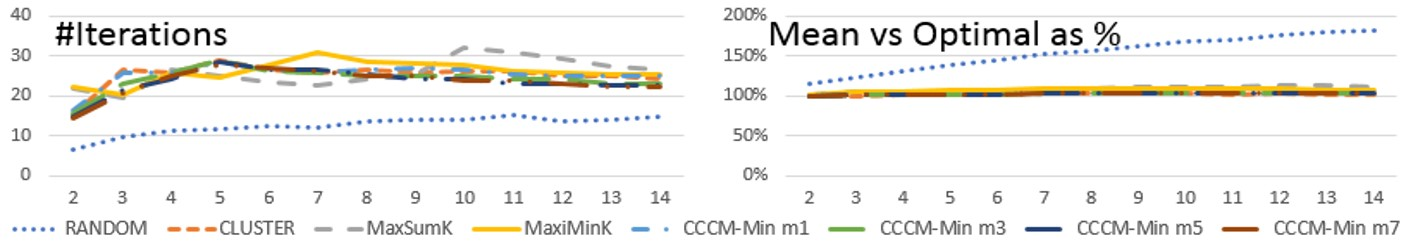
\includegraphics[width=\linewidth]{MiceIters.jpg}
  \caption{UCI Mice Protein: a) \#Iterations, b) Mean vs Optimal.}
  \label{fig:miceIters}
\end{figure}

\begin{figure}
  \centering
  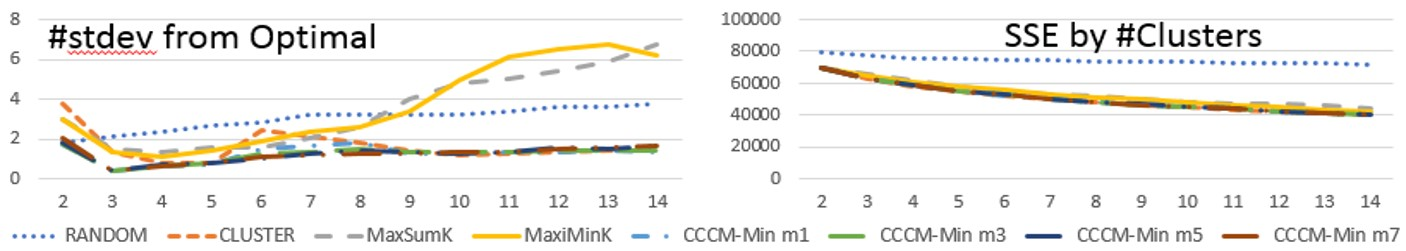
\includegraphics[width=\linewidth]{MiceStdev.jpg}
  \caption{UCI Mice Protein: a) \#Stdev Away from Optimal, b) SSE by \#Clusters.}
  \label{fig:miceStdev}
\end{figure}


\begin{figure}
  \centering
  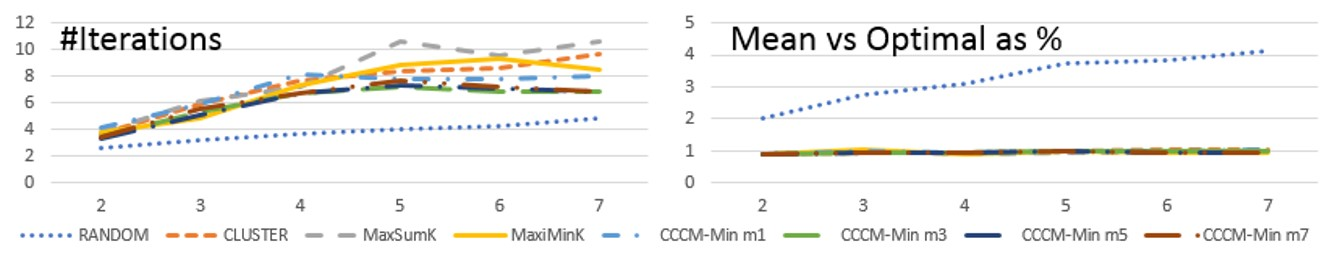
\includegraphics[width=\linewidth]{IrisIters.jpg}
  \caption{UCI Iris: a) \#Iterations, b) Mean vs Optimal.}
  \label{fig:irisIters}
\end{figure}

\begin{figure}
  \centering
  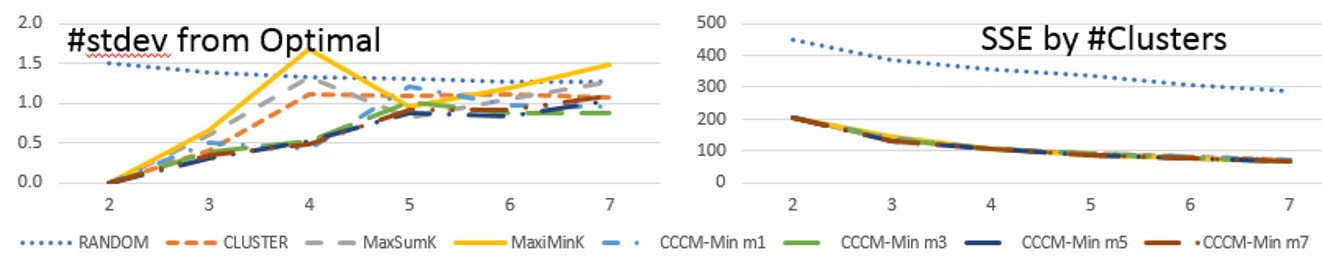
\includegraphics[width=\linewidth]{IrisStdev.jpg}
  \caption{UCI Iris: a) \#Stdev Away from Optimal, b) SSE by \#Clusters.}
  \label{fig:irisStdev}
\end{figure}

Having few clusters in few dimensions with little or no overlap provides fertile ground for any initialization method to find a high-quality result.  However, the results show that the initialization choice affects both the overall quality and performance, even when there are few clusters.  In the tested dimensions, the CCCM initialization method offers $\sim$$95\%$ improvement in quality and $\sim$$50\%$ improvement in relative performance compared to standard initialization methods, which further improves as the number of points or the number of true clusters increase.  CCCM appears to be consistent in both quality and performance even with an increase in the number of dimensions, number of points, and the number of clusters.

Values tested for the configurable multiplier $m$ ranged from 1 to 7.  With each increase in $m$, both the quality and performance were improved, due to the increased probability in having each cluster represented with an initial centroid.  The empirical tests show that $m=6$ is sufficient to achieve quality within $2\%$ of optimal, through $K=100$, and that $m=7$ drives the quality to within $1\%$ of optimal.  A potential need exists to increase $m$ beyond 7.  Based on the empirical data reviewed, a simple formula of $m=6 + 1 per 100 clusters$ seems appropriate.  The relative cost of increasing $m$ is small.  It should be noted that even with an increase in $m$ or $K$, the setup computation cost is far less than a single iteration against all N points.

The result for CCCM-Rnd, -Min, and -MxMn were sufficiently close to one another that, for general purposes, any of the three will suffice.  The difference between the three is less than $0.1\%$.

With linearly separable clusters, both the quality and performance of CCCM continue to be superior to the older methods.  However, intertwined clusters still create a significant problem.

\section{Further Investigation}

This study did not investigate skewed distributions.  It is expected that the extremely large clusters may overshadow the smallest clusters, such that they are not represented in the initial selection of points.  The maximum distance requirements will mitigate this issue, but one should consider removing such extreme clusters and re-running on the remainder.

\section{Conclusion}

The CCCM approach to initialize the K-Means algorithm based on choosing potential initial centers from a small subset of the actual data points and maximizing the minimums of the cross-centroid costs to select the initial K points appears to provide a more effective, more efficient, and more robust initialization.
Figure \ref{fig:stdevAway13D}, the stdev-away-from-optimal chart, shows that the optimal is within reach of CCCM while improbable that using another initialization method would ever achieve the optimal solution.
The $\sim$$95\%$ quality improvement, often using $\sim$$50\%$ fewer iterations means that one could eliminate the need for multiple executions of K-Means to find high quality clustering.  The quality of the results, the performance effort, and the ability to correctly and efficiently identify the size of K have implications for big data sets.

\section*{References}

\begin{thebibliography}{9}
\bibitem{bradley} 
Bradley, P.S., Fayyad, U.M.
\textit{Refining Initial Points for K-Means Clustering}.
Microsoft Technical Report (MSR-TR-98-36), 1998

\bibitem{celebi} 
Celebi, M.E., Kingravi, H.A., Vela, P.A. 
\textit{A Comparative Study of Efficient Initialization Methods for the K-MeansClustering Algorithm}.
Expert Systems with Applications, 40(1):200-210, 2013.

\bibitem{forgy} 
Forgy, E.W. 
\textit{Cluster Analysis of Multivariate data: efficiency vs. Interpretability of Classifications}.
Biometrics, Vol. 21:768-769, 1965.

\bibitem{haraty} 
Haraty, R.D., Dimishkieh M., Masud M.
\textit{An Enhanced k-Means Clustering Algorithm for Pattern Discovery in Healthcare Data}.
International Journal of Distributed Sensor Networks, 11(6), 2015.

\bibitem{jancey} 
Jancey, R.C.
\textit{Multidimensional Group Analysis}.
Australian Journal of Botany, 14(1):127–130, 1966.

\bibitem{leskovec} 
Leskovec, J., Rajaraman, A. 
Stanford University - CS 345A - Data Mining - Clustering Algorithms,
\texttt{https://web.stanford.edu/class/cs345a/slides/12-clustering.pdf}

\bibitem{macqueen} 
MacQueen, J. 
\textit{Some Methods for Classification and Analysis of Multivariate Observations}.
Proceedings of the 5th Berkeley Symposium on Mathematical Statistics and Probability, 281–297, 1967.

\bibitem{ng} 
Ng, A.
Lecture 13.2 — Clustering | KMeans Algorithm — [ Machine Learning | Andrew Ng ]
\\\texttt{https://www.youtube.com/watch?v=hDmNF9JG3lo}

\bibitem{pena} 
Peña, J.A. 
\textit{An empirical comparison of four initialization methods for the K-Means algorithm}.
Pattern Recognition Letters, 20(10):1027-1040, 1999.

\bibitem{UC} 
UC,
UC Business Analytics R Programming Guide,
\\\texttt{https://uc-r.github.io/kmeans\_clustering}

\bibitem{UCIIris} 
UCI Machine Learning Repository,
Iris Data Set,
\\\texttt{http://archive.ics.uci.edu/ml/datasets/iris}

\bibitem{UCIMice} 
UCI Machine Learning Repository,
Mice Protein Expression Data Set,
\\\texttt{https://archive.ics.uci.edu/ml/datasets/Mice+Protein+Expression}

\bibitem{yse} 
Yse, D.L. 
The Anatomy of K-Means Clustering,
\\\texttt{https://opendatascience.com/the-anatomy-of-k-means-clustering}


\end{thebibliography}

\end{document}
